%%%% fatec-article.tex, 2024/03/10

%% Classe de documento
\documentclass[
  a4paper,%% Tamanho de papel: a4paper, letterpaper (^), etc.
  12pt,%% Tamanho de fonte: 10pt (^), 11pt, 12pt, etc.
  english,%% Idioma secundário (penúltimo) (>)
  brazilian,%% Idioma primário (último) (>)
]{article}

%% Pacotes utilizados
\usepackage[]{fatec-article}
\usepackage{float}
\Author{1}{Name={Estevam R.\\Frazão L.\\Lucca de B.\\ Flávia A. \\Lima L.}}

\Author{2}{Name={\{ ricardo.conceicao@fatec.sp.gov.br \}\\ \{ Lucas.guimaraes11@fatec.sp.gov.br\} \\ \{ Bruno.miranda19@fatec.sp.gov.br\} \\ \{ ana.goncalves60@fatec.sp.gov.br \}  \\ \{ Leonardo.lima83@fatec.sp.gov.br\}}}

%% Definição das palavras-chaves/keywords
\Keyword{1}{Artigo}{Article}
\Keyword{2}{Latex}{Latex}
\Keyword{3}{Informática}{Informatic}

%%%% Resumo no idioma primário (brazilian)
\begin{Abstract}[brazilian]%% Idioma (brazilian ou english)
  O Projeto Classificação de Bacteriose nas Folhas da Mandioca, Orientado por Aprendizagem Profunda tem como objetivo desenvolver um aplicativo de inteligência artificial (IA) para detectar as probabilidades da infecção por Xanthomonas phaseoli pv. manihotis (Xpm) em folhas de mandioca. Utilizando técnicas de deep learning, o aplicativo permitirá que os usuários capturem imagens das plantas ou enviem imagens armazenadas em seus dispositivos, com intuito de serem analisadas de forma eficaz pela IA do aplicativo, onde será exibido o grau de infecção da planta, fornecendo informações precisas e com agilidade. Além disso, o projeto busca criar um sistema de mapeamento que ajudará na identificação de áreas mais vulneráveis, possibilitando intervenções direcionadas e a melhoria das práticas agrícolas.
A implementação deste aplicativo visa não apenas facilitar o monitoramento da saúde das plantações, mas também dar informações aos agricultores com dados que podem ser utilizados para tomar decisões, a fim de ser orientado por um profissional futuramente. A capacidade de detectar infecções de maneira rápida e eficiente é crucial para a diminuição dos danos causados pela bacteriose, promovendo a sustentabilidade da produção de mandioca e contribuindo para a segurança alimentar nas comunidades afetadas.

\end{Abstract}

%%%% Resumo no idioma secundário (english)
\begin{Abstract}[english]%% Idioma (brazilian ou english)
  The Project Classification of Bacteriosis in Cassava Leaves, Guided by Deep Learning aims to develop an artificial intelligence (AI) application to detect the probabilities of infection by Xanthomonas phaseoli pv. manihotis (Xpm) in cassava leaves. Using deep learning techniques, the application will allow users to capture images of plants or send images stored on their devices, in order to be analyzed effectively by the application's AI, where the degree of infection of the plant will be displayed, providing accurate information and with agility. Furthermore, the project seeks to create a mapping system that will help identify the most vulnerable areas, enabling targeted interventions and the improvement of agricultural practices.
  The implementation of this application aims to not only facilitate monitoring the health of crops, but also provide information to farmers with data that can be used to make decisions, in order to be guided by a professional in the future. The ability to detect infections quickly and efficiently is crucial to reducing the damage caused by bacteriosis, promoting the sustainability of cassava production and contributing to food security in affected communities.
\end{Abstract}

%% Processamento de entradas (itens) do índice remissivo (makeindex)
\makeindex%

%% Arquivo(s) de referências
\addbibresource{fatec-article.bib}

%% Início do documento
\begin{document}

% Seções e subseções
%\section{Título de Seção Primária}%

%\subsection{Título de Seção Secundária}%

%\subsubsection{Título de Seção Terciária}%

%\paragraph{Título de seção quaternária}%

%\subparagraph{Título de seção quinária}%

\section*{Introdução}%
\label{sect:intro}
A ONU (Organizações das Nações Unidas) tem como proposta os objetivos de desenvolvimento sustentável (ODS) e um dos seus objetivos é a “Vida Sobre a Terra”, com a expectativa de: proteger, recuperar e promover o uso sustentável dos ecossistemas terrestres, gerir de forma sustentável as florestas, combater a desertificação, deter e reverter a degradação da terra e deter a perda.  O Brasil tem grande destaque como um dos principais países exportadores agrícolas do planeta.

Em 2023, o país teve uma alta de 4,8\% em relação ao ano anterior, e, somadas, as exportações chegaram ao valor de US\$166,55 bilhões, segundo dados do Ministério da Agricultura e Pecuária \textcite{MAPA:11}. No Brasil, a mandioca (Manihot esculenta Crantz) é uma das plantações mais significativas em termos de volume de produção, ficando atrás apenas da cana-de-açúcar \cite{FURLANETO}. 

Pesquisas realizadas pela CONAB mostram que o Brasil é o quarto maior exportador de mandioca na américa latina. O Estado de São Paulo possui uma área plantada de 51 mil hectares, posicionando-se como o sexto maior produtor de mandioca no país, (INSTITUTO DE ECONOMIA AGRÍCOLA),\textcite{CONAB}. Na região do Vale do Ribeira encontra-se um número significativo na produção de Mandioca onde é cultivada e comercializada internamente por povos Quilombolas. Os quilombolas se localizam em áreas remotas ao longo da Bacia do Rio Ribeira de Iguape (sul do Brasil), cobertas pela vegetação da Mata Atlântica, um dos hotspots de biodiversidade do mundo, desde os primórdios da ocupação (século XVIII), os quilombolas têm sido historicamente dependentes do cultivo de arroz, milho, mandioca e feijão \cite{Prado}.

Esta importante cultura está ameaçada por diversas pragas que impactam a produtividade, e entre esses problemas, as bacterioses são uma das principais preocupações. As bacterioses (doenças originadas por bactérias), recebem uma posição de destaque dentre essas pragas e podem ser nocivas à plantações, podendo acarretar até o desfalecimento das plantas se não forem previamente identificadas e tratadas \textcite{Embrapa}. Dentre os patógenos bacterianos, o Xanthomonas phaseoli pv. manihotis (Xpm) atraí atenção significativa da comunidade científica devido ao seu comportamento vascular e sistêmico, que lhe confere um alto potencial de causar danos significativos em plantações de mandioca, especialmente em regiões tropicais, atraindo assim a relevância científica em todo mundo \cite{MANSFIELD}.

A bacteriose Xanthomonas afeta cerca de 30\% de toda produção de mandioca \textcite{Germoplasma}. O prejuízo na produção das raízes pode afetar em até 70\% do seu peso, tornando a produção inviável quando não se tem o controle dessa doença \textcite{Embrapa}. Um dos problemas enfrentados é a falta de informações da incidência dessas bacteriose, embora mais patógenos bacterianos infectam a mandioca, as informações na literatura são escassas (Cassava diseases caused by Xanthomonas phaseoli pv. manihotis and Xanthomonas cassavae., 2021)\textcite{Cassava1999}. Com base nas pesquisas apontadas anteriormente é notório a preocupação com relação às bacterioses nas plantações e seus impactos no mundo agrícola. 

Com o objetivo de identificar a bacteriose e realizar seu mapeamento, considerou-se a criação de um aplicativo suportado por uma Inteligência Artificial (IA) por meio de Redes Neurais Artificiais. A Deep Learning é uma subcategoria da inteligência artificial que envolve o treinamento de redes neurais profundas para reconhecer padrões complexos e aprender continuamente a partir de grandes volumes de dados. Após o processo de treinamento, essas redes são capazes de executar tarefas semelhantes com as de seres humanos, sendo uma delas analisar imagens com alta precisão. Este aplicativo visa monitorar e, trazer, em probabilidade, o grau da bacteriose Xanthomonas na planta, visto que a bacteriose da mandioca, causada por Xanthomonas phaseoli pv. manihotis, é uma das doenças mais importantes que afetam a produção de mandioca no mundo.(Scielo.,Bactérias endofíticas Klebsiella controlam a bacteriose da mandioca na Amazônia Oriental., 2024)\cite{Klebsiella}.





\section*{OBJETIVO} \label{sect:obj}

Este estudo visa desenvolver um sistema baseado em inteligência artificial para a detecção e mapeamento da infecção por Xanthomonas phaseoli pv. manihotis em folhas de mandioca. Utilizando a tecnologia Deep Learning, o sistema irá analisar imagens das folhas para identificar e classificar o grau de infecção com base em probabilidades. Além disso, pretende-se integrar os dados de infecção com informações, a fim de mapear a distribuição da praga na região do Vale do Ribeira.
Objetivo Específico:
Mapear a doença, realizando levantamentos da incidência da bacteriose Xanthomonas phaseoli pv. manihotis nas plantações de mandioca no Vale do Ribeira, identificando áreas de maior impacto.
Desenvolver um aplicativo baseado em Inteligência Artificial que utilize Deep Learning para identificar e prever a ocorrência da bacteriose em plantações de mandioca, possibilitando maior agilidade no reconhecimento da bacteriose em grandes áreas de plantações.





\section*{ESTADO DA ARTE} \label{sect:estadoarte}

O uso de Inteligência Artificial para resolução de problemas complexos vem ganhando força no mundo inteiro. Na agricultura, um sistema que utiliza visão computacional para analisar uma plantação e saber o seu estado requer altos investimentos. Entretanto, o uso de redes neurais pode resultar em custos reduzidos, especialmente quando se considera que apenas um dispositivo móvel, como um smartphone, é suficiente para a captura e análise de imagens.

No artigo Utilização de IA para Controle de Pragas na Agricultura (\textcite{CPA2022}), observa-se o uso de Machine Learning. Esse projeto tem como objetivo utilizar soluções de Machine Learning para coletar e analisar imagens que mostram as condições das folhas da soja e identificar se há ou não alguma praga com base na imagem.

Um método semelhante a esse é o EfficientNet, que é uma subcategoria do Machine Learning. O EfficientNet é uma arquitetura específica de Redes Neurais Convolucionais (CNN) desenvolvida para otimizar o desempenho em tarefas de visão computacional. O projeto Método de detecção de doenças da mandioca baseado no EfficientNet utiliza esse método e se aprofunda no uso de métodos de aprendizagem profunda . O foco principal do projeto mencionado é categorizar doenças foliares usando imagens do conjunto de dados Kaggle \cite{Leaf}.

De forma semelhante, o projeto Classificação de doenças foliares de mandioca, orientado por Aprendizagem Profunda \textcite{EfficientNet}, propõe usar o espaço de cores HSV além do EfficientNet para realizar a tarefa de identificação da praga na plantação de mandioca. Converter imagens para o espaço HSV como parte do pré-processamento pode simplificar o treinamento de modelos de machine learning e EfficientNet, especialmente quando o modelo precisa aprender características específicas da cor.

O Machine Learning mostrado anteriormente nos artigos demonstra ser uma boa opção quando se trata de avaliar imagens; porém, a Deep Learning possui uma maior capacidade de capturar padrões complexos. Sendo assim, o projeto Classificação de Bacteriose nas Folhas da Mandioca visa utilizar a Deep Learning para identificar a bacteriose Xanthomonas phaseoli. Como existem diversas bacterioses semelhantes a Xanthomonas phaseoli, a estrutura fornecida pela Machine Learning pode não ser suficiente para diferenciar essas formas da bacteriose, resultando em uma menor precisão na identificação.

\section*{METODOLOGIA} \label{sect:metodologia}

    \begin{figure}[H]
    \centering
    \caption{Exemplo de figura}%
    \label{fig:Metodologia.PNG}
    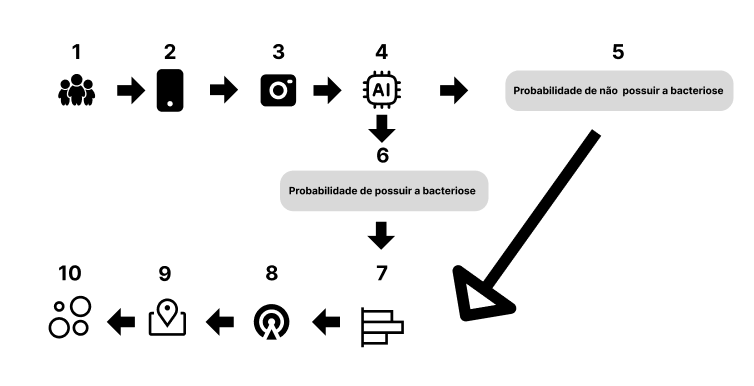
\includegraphics[scale=0.9]{Metodologia.PNG}
    \SourceOrNote{Autoria Própria (2024)}
    \end{figure}

Imagem 1 e 2:
Inicialmente, o usuário acessa o aplicativo e realiza seu cadastro fornecendo informações pessoais básicas. Esse cadastro é necessário para permitir o uso das funcionalidades do sistema e o armazenamento de dados associados.

Imagem 3:
Após o login do usuário, o mesmo interage com uma interface que permite o acesso à câmera do dispositivo. Essa etapa é fundamental para a captura da imagem da folha de mandioca, que futuramente será analisada a presença da bacteriose na folha.

Imagem 4:
O usuário realiza a captura de uma imagem da folha de mandioca, que deve seguir orientações específicas fornecidas pelo aplicativo, como foco e iluminação adequados, para garantir a maior precisão na análise.

Imagem 5:
Após a captura da imagem, o sistema de inteligência artificial processa a imagem e calcula a probabilidade de presença da bacteriose Xanthomonas paesoli. Isso supondo que o algoritmo utilizado foi treinado com um banco de dados de imagens previamente classificadas, possibilitando uma análise precisa.

Imagem 6:
Caso a probabilidade de presença da bacteriose seja baixa, o sistema informa ao usuário que a planta está saudável, indicando a confiança dessa análise com base nos resultados do modelo.
Imagem 7:
Se a probabilidade de presença da bacteriose for elevada, o aplicativo informa o usuário sobre a possível presença da infecção.

Imagem 8:
Em caso de detecção da bacteriose, o sistema realiza o envio dos dados de geolocalização, capturados via GPS, para identificar o local exato onde a foto foi tirada.

Imagem 9:
O GPS do dispositivo registra com precisão a localização da planta examinada, armazenando as coordenadas geográficas no banco de dados para análises posteriores.

Imagem 10:
Os dados de geolocalização são processados para gerar um mapa de calor que representa as áreas com maior incidência da bacteriose. Este mapa visa ser atualizado em tempo real, com base nas imagens capturadas e processadas em diferentes localidades.


\section*{RESULTADOS PRELIMINARES}\label{sect:resultados}

Com o progresso do projeto, alcançamos os seguintes resultados: a prototipação das telas para dispositivos móveis utilizando o software Figma, a construção do site com a ferramenta Oracle APEX (uma plataforma que facilita o desenvolvimento de aplicações web), a elaboração do Diagrama de Caso de Uso (DCU), a Modelagem do Banco de Dados (MBD), tanto na perspectiva lógica quanto conceitual, a definição do Escopo de Redes e a criação do Modelo de Negócios no Canvas Sebrae.

\textbf{Prototipação do Aplicativo}

Com ajuda do Figma fizemos a primeira tela, que é chamada de Splash Screen (tela inicial), nela voce o usuário pode cadastrar uma conta ou entrar com uma conta já existente conforme ilustrado na \Cref{phot:pg-2}.

\begin{figure}[H]
    \centering
    \SetCaptionWidth{\ifbool{@LayoutA}{0.6}{0.72}\linewidth}
    \caption{Splash Screen}%
    \label{phot:pg-2}
    \savebox0{
\includegraphics[scale=0.5]{Illustrations/Login.jpg}}
    \usebox0%
    \SourceOrNote{Autoria Própria (2024)}
\end{figure}

    Já na tela principal do aplicativo o usuário pode escolher três funções interativas principais através de uma tela rolável, sendo elas: Escanear Folha, Meus Arquivos e Indices Locais como mostrado na   \Cref{phot:pg-3}.

    \begin{figure}[H]
        \centering
        \SetCaptionWidth{\ifbool{@LayoutA}{0.6}{0.72}\linewidth}
        \caption{Main Screen (Tela Principal)}%
        \label{phot:pg-3}
        \savebox0{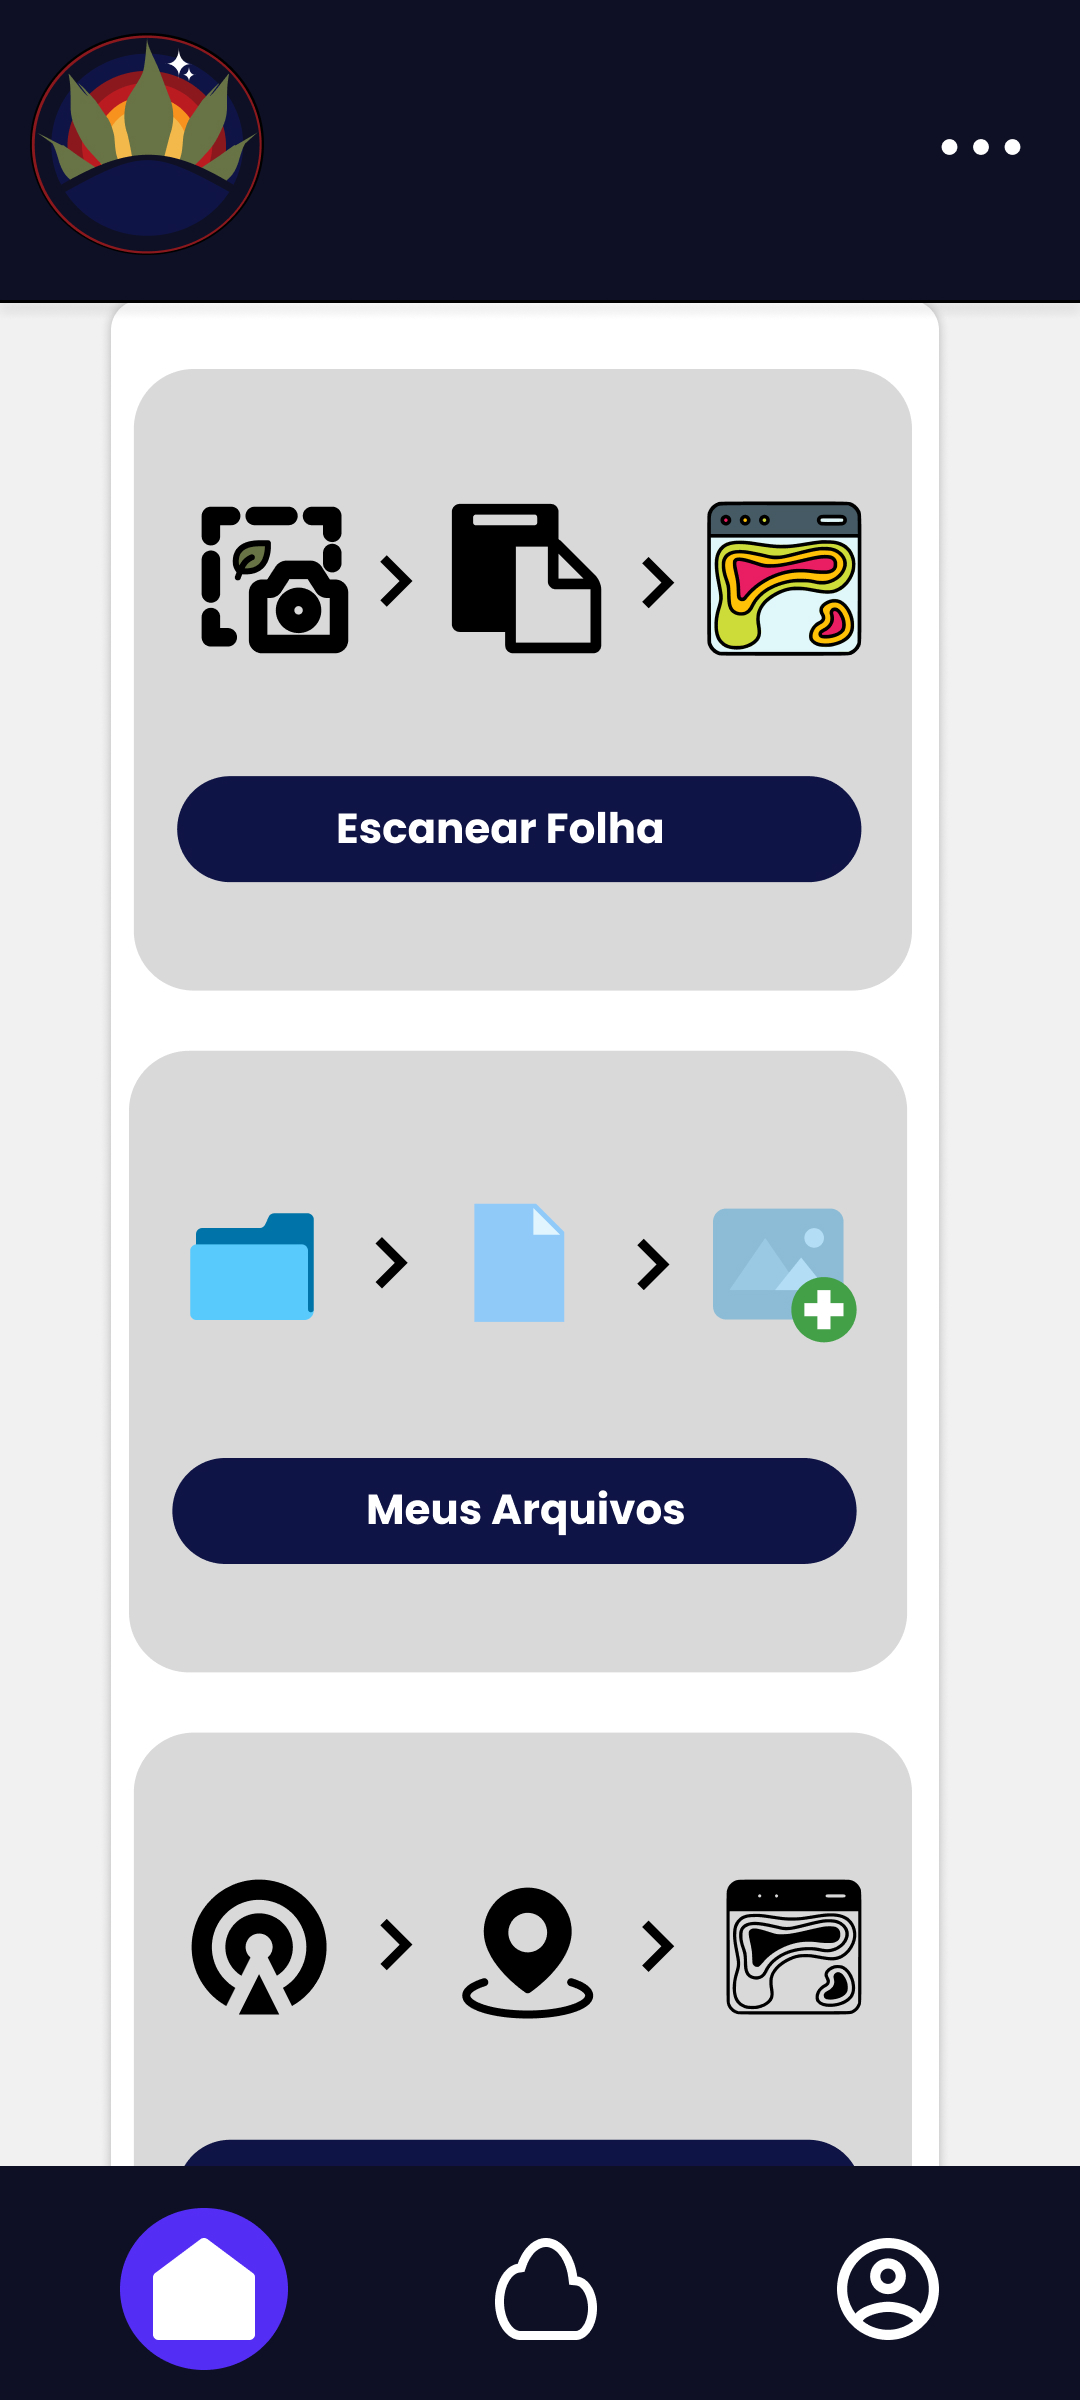
\includegraphics[scale=0.5]{Illustrations/PRINCIPAL.jpg}}
        \usebox0%
        \SourceOrNote{Autoria Própria (2024)}
    \end{figure}

    Após apertar para Escanear a folha o aplicativo leva o usuário para tela de escaneamento, onde uma Inteligência Artificial analisa a imagem tirada pelo usuário \Cref{phot:pg-4}.   

    \begin{figure}[H]
        \centering
        \SetCaptionWidth{\ifbool{@LayoutA}{0.6}{0.72}\linewidth}
        \caption{Tela de Escaneamento (Scan Screen)}%
        \label{phot:pg-4}
        \savebox0{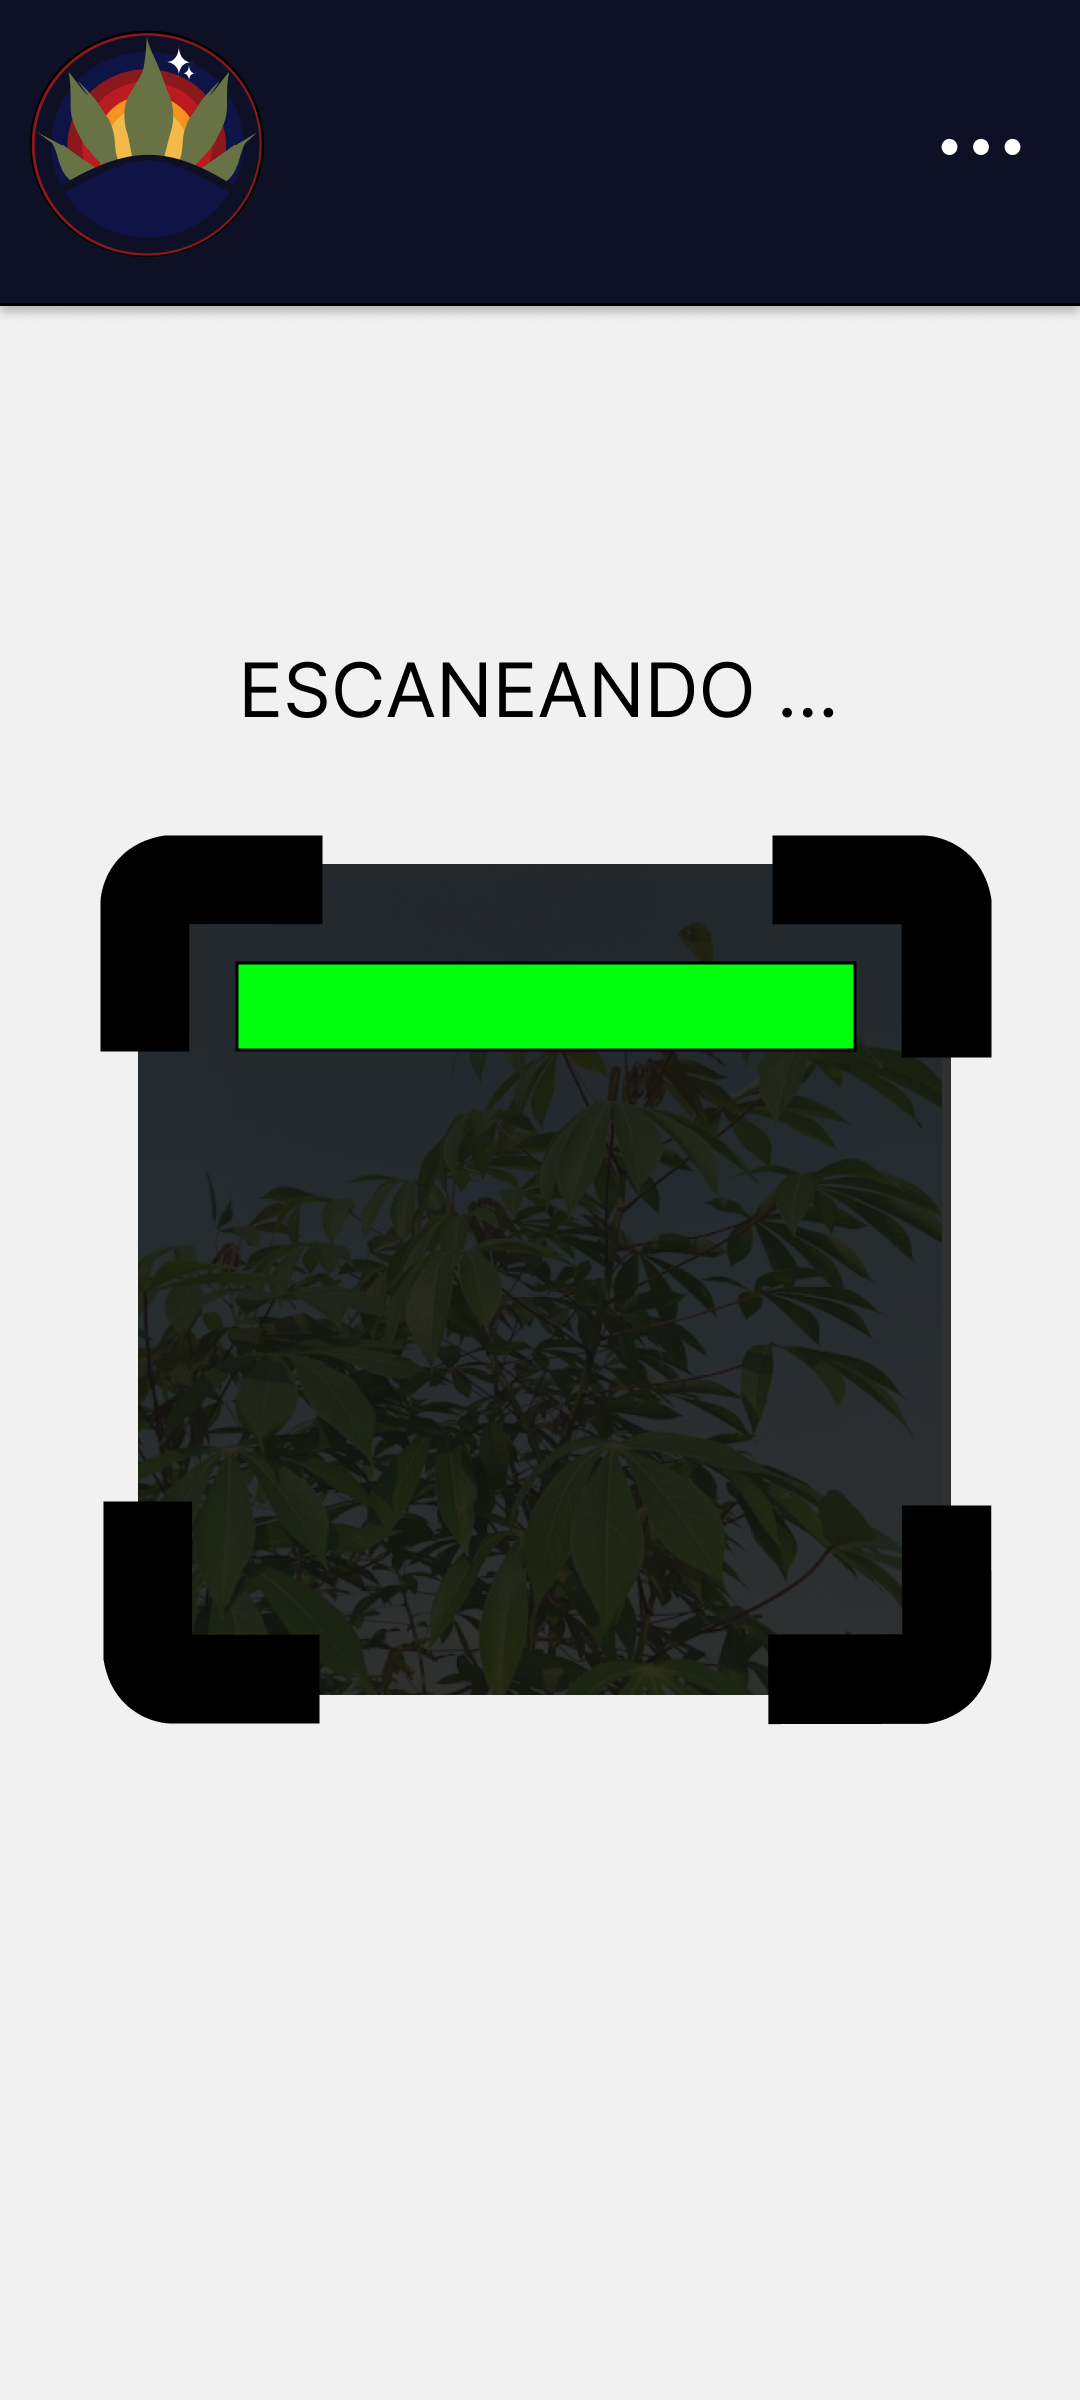
\includegraphics[scale=0.5]{Illustrations/Identificacao.png}}
        \usebox0%
        \SourceOrNote{Autoria Própria (2024)}
    \end{figure}

    Em seguida é mostrado na tela a probabilidade da folha da mandioca possuir a bacteriose, em uma seção onde é mostrado em detalhes o que aconteceu com a planta com a ajuda da analise fornecida pela IA (Inteligência Artificial); o usuário também pode salvar a sua localização para registrar no mapa de calor da região \Cref{phot:pg-5}.
    \begin{figure}[H]
        \centering
        \SetCaptionWidth{\ifbool{@LayoutA}{0.6}{0.72}\linewidth}
        \caption{Tela Relatório (Report Screen)}%
        \label{phot:pg-5}
        \savebox0{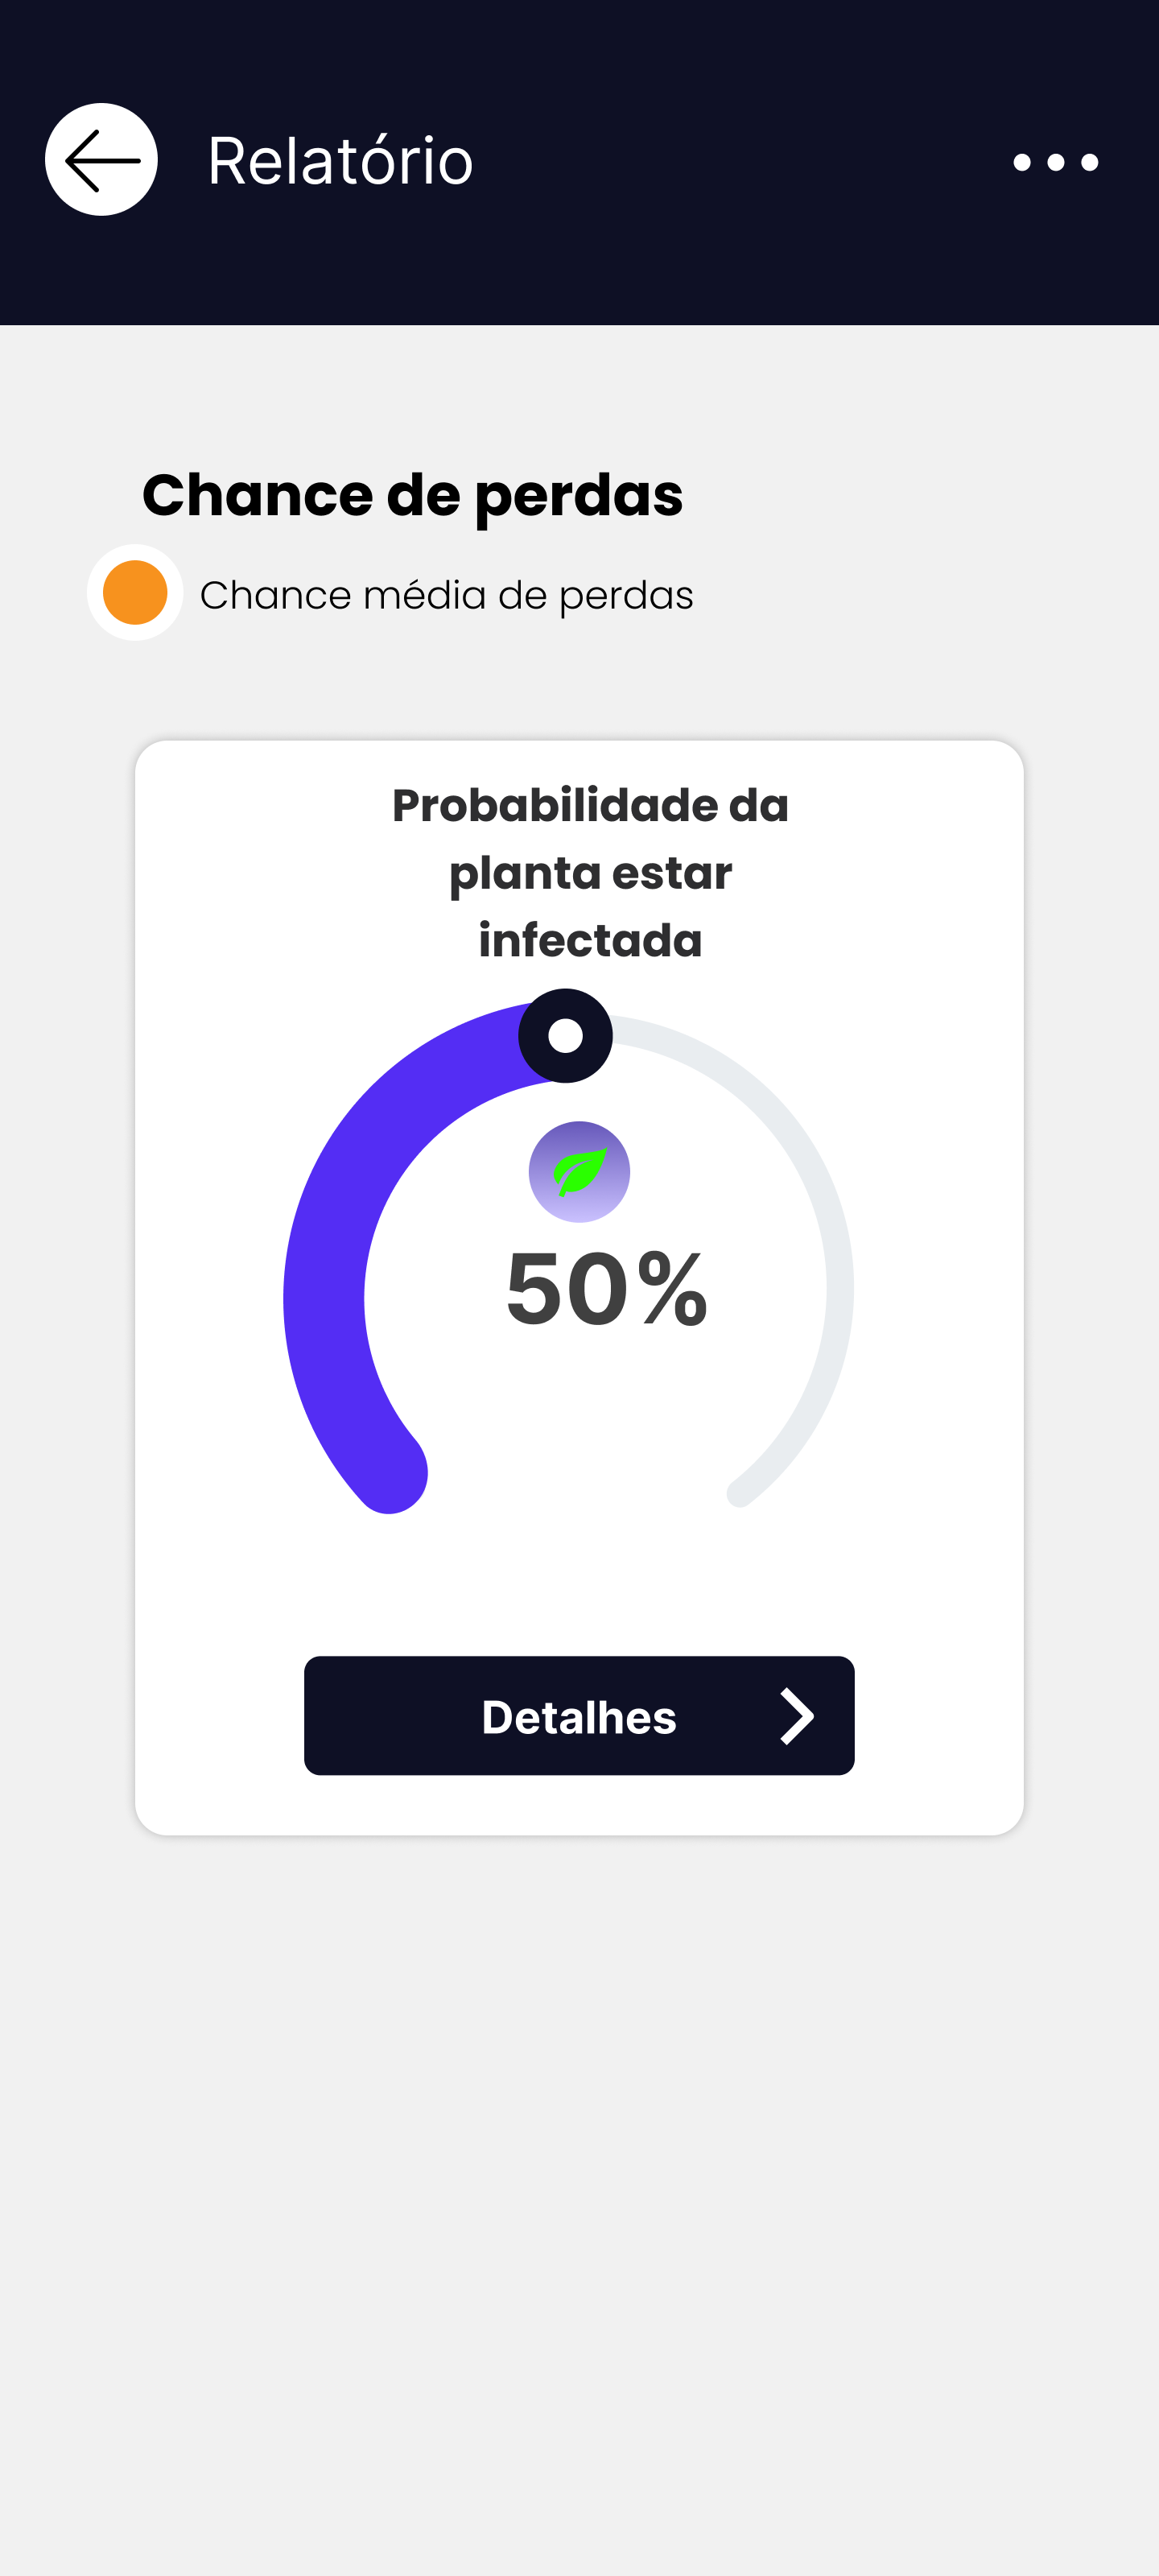
\includegraphics[scale=0.5]{Illustrations/Relatorio_2.png}}
        \usebox0%
        \SourceOrNote{Autoria Própria (2024)}
    \end{figure}

    Após o usuário salvar a imagem no mapa de calor ele é encaminhado para tela de Índices Locais onde será mostrado o mapa de calor da região \Cref{phot:pg-6}.
    
    \begin{figure}[H]
        \centering
        \SetCaptionWidth{\ifbool{@LayoutA}{0.6}{0.72}\linewidth}
        \caption{Mapa de Calor (Heat Map)}%
        \label{phot:pg-6}
        \savebox0{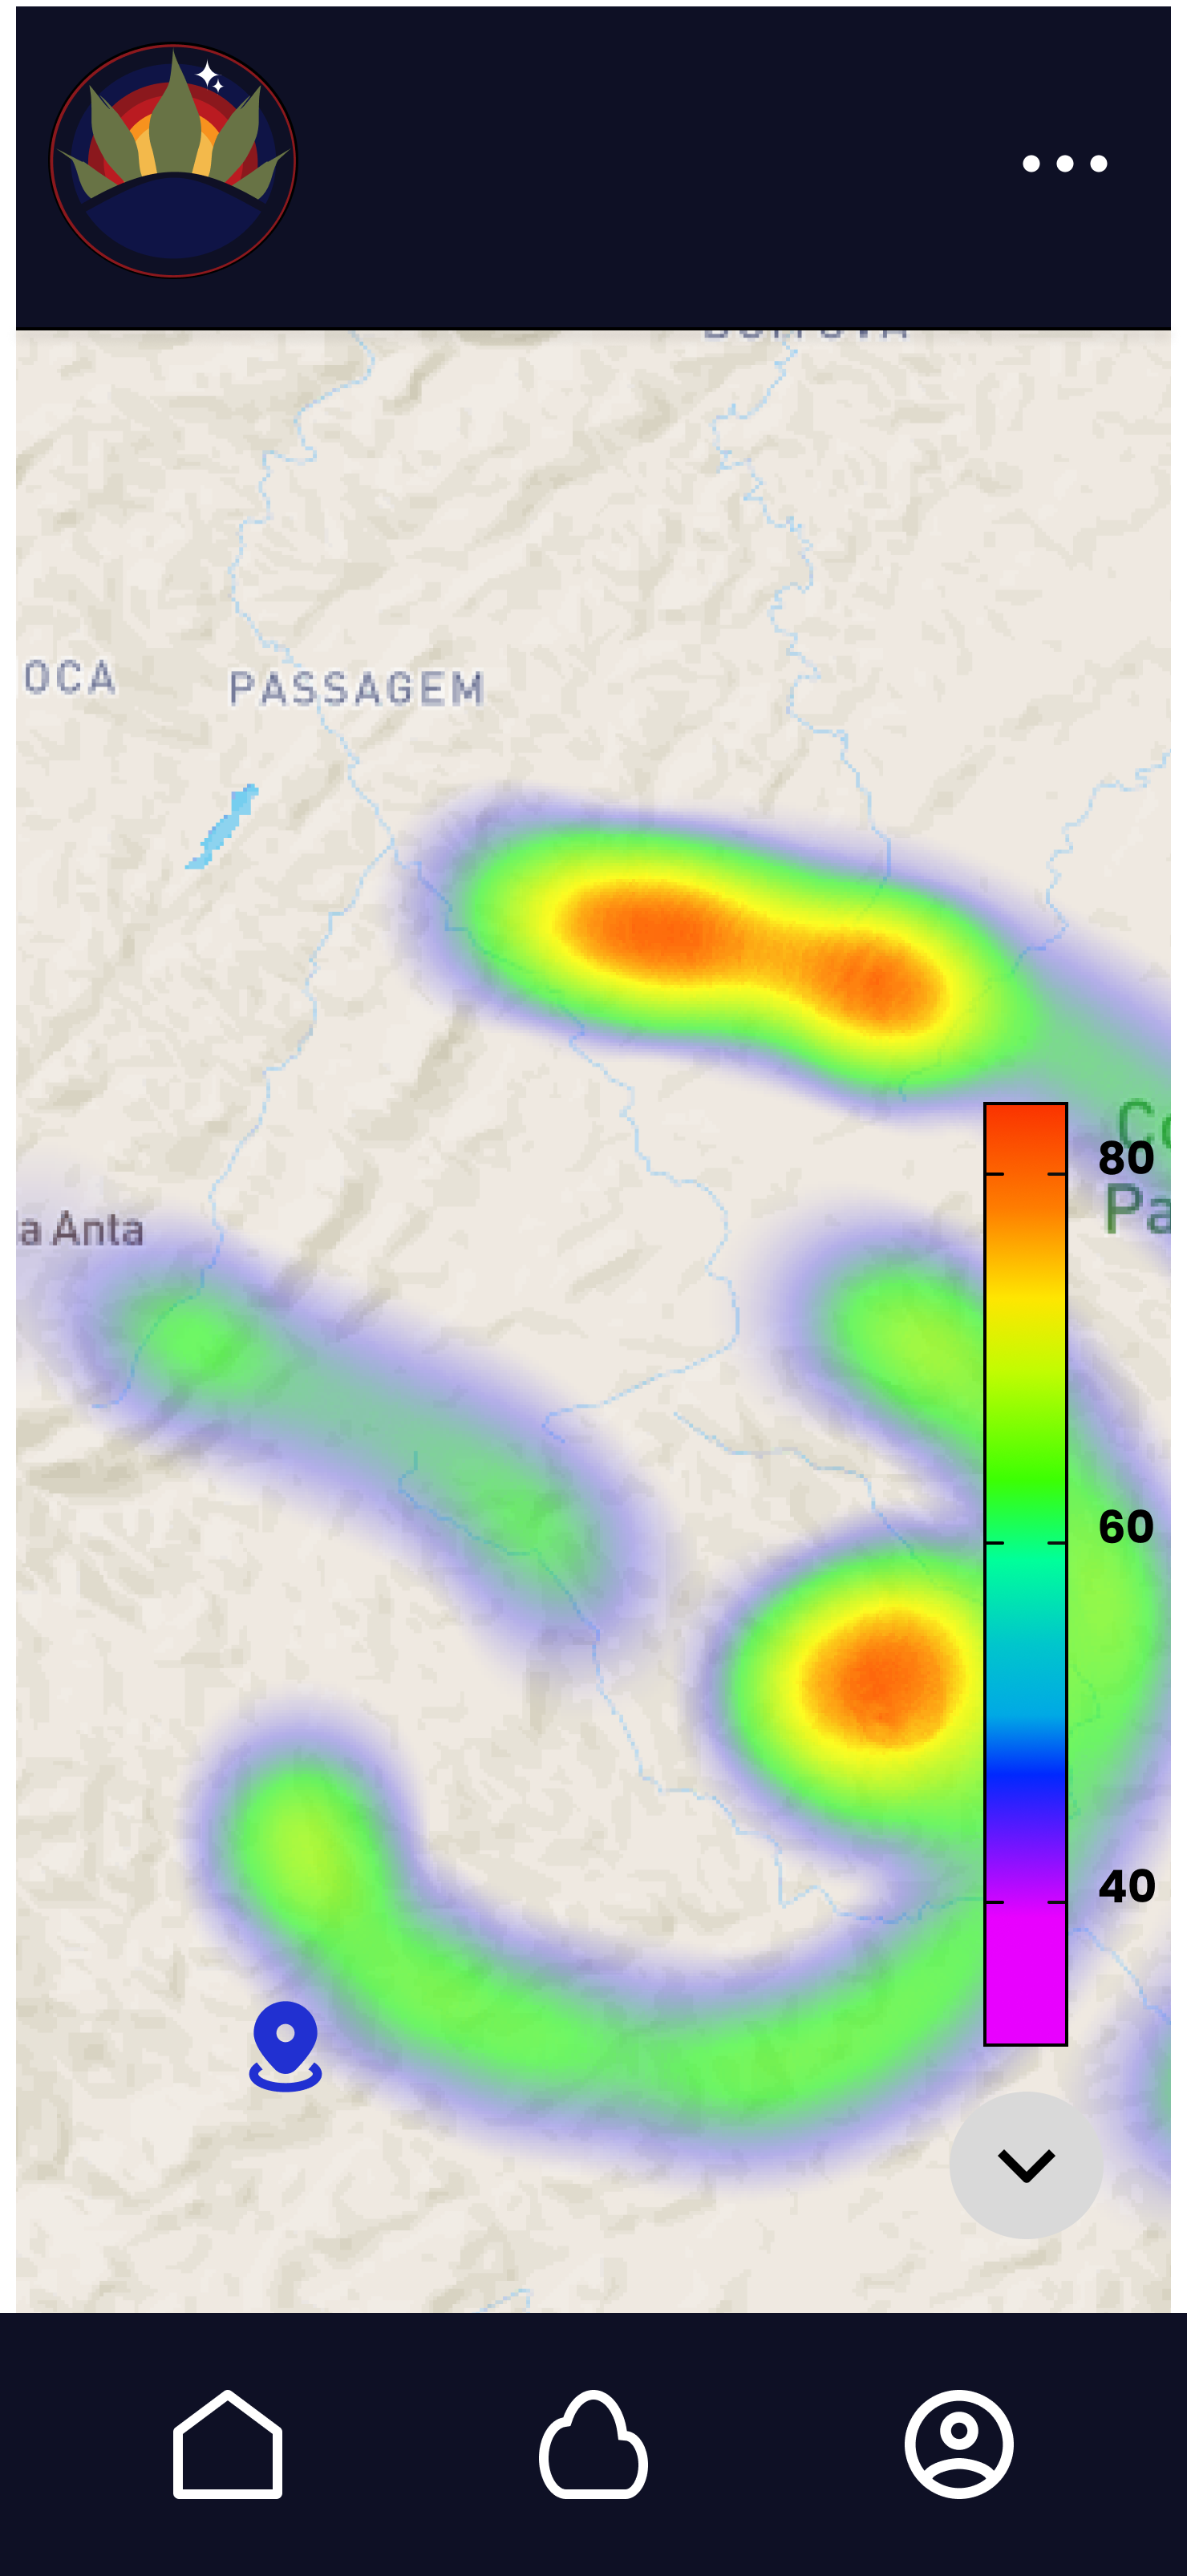
\includegraphics[scale=0.5]{Illustrations/mapa_calor.png}}
        \usebox0%
        \SourceOrNote{Autoria Própria (2024)}
    \end{figure}

    \textbf{APEX}
    
    O APEX é uma plataforma de desenvolvimento da Oracle que possui o intuito de criar aplicativos web de forma rápida e sem necessidade de conhecimentos profundos em programação. O APEX oferece uma interface gráfica para o desenvolvimento de aplicações que integram facilmente com bancos de dados Oracle, ideal para criar painéis, formulários, relatórios, e outras funcionalidades interativas.

    A primeira tela criada no APEX foi a tela de início, que é exibida quando o proprietário acessa o sistema. Essa tela inicial serve como ponto de entrada e fornece uma visão geral do sistema, permitindo uma navegação rápida para as funcionalidades principais, como mostrado na ilustração \Cref{phot:pg-15}.

    \begin{figure}[H]
        \centering
        \SetCaptionWidth{\ifbool{@LayoutA}{0.6}{0.72}\linewidth}
        \caption{Tela de início(APEX)}%
        \label{phot:pg-15}
        \savebox0{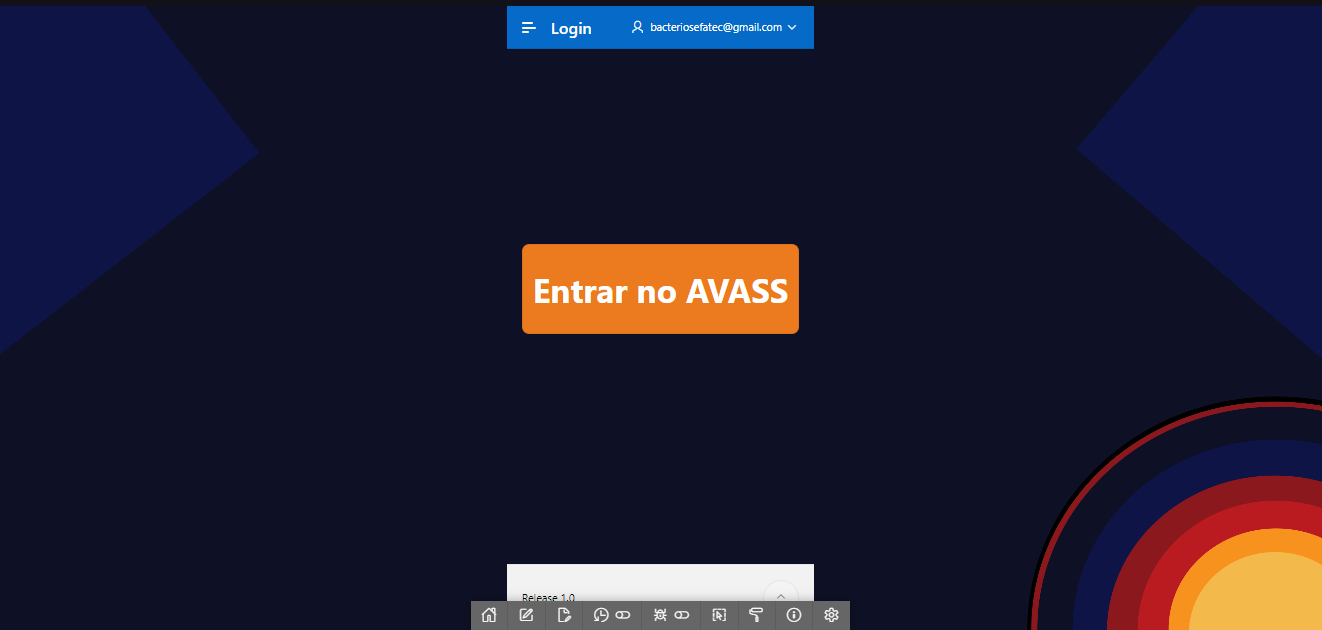
\includegraphics[scale=0.5]{Illustrations/Tela1_APEX.png}}
        \usebox0%
        \SourceOrNote{Autoria Própria (2024)}
    \end{figure}

    Na Figura \Cref{phot:pg-15} é mostrado a tela de login onde o proprietário entra com sua conta.

    \begin{figure}[H]
        \centering
        \SetCaptionWidth{\ifbool{@LayoutA}{0.6}{0.72}\linewidth}
        \caption{Tela de login(APEX)}%
        \label{phot:pg-15}
        \savebox0{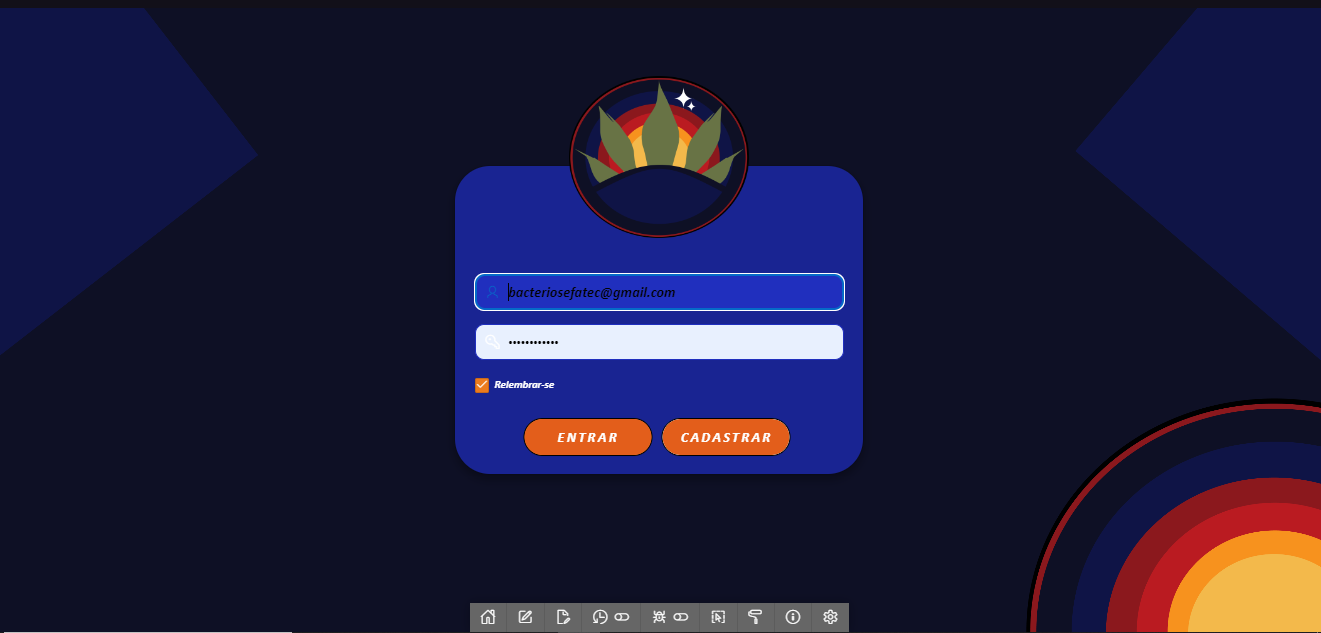
\includegraphics[scale=0.5]{Illustrations/tela2_APEX.png}}
        \usebox0%
        \SourceOrNote{Autoria Própria (2024)}
    \end{figure}

    Após o proprietário entrar, ele é direcionado para a tela do mapa de calor, onde pode visualizar as estatísticas clicando no botão "Ver nas tabelas". \Cref{phot:pg-16}

    
    \begin{figure}[H]
        \centering
        \SetCaptionWidth{\ifbool{@LayoutA}{0.6}{0.72}\linewidth}
        \caption{Mapa de Calor(APEX)}%
        \label{phot:pg-16}
        \savebox0{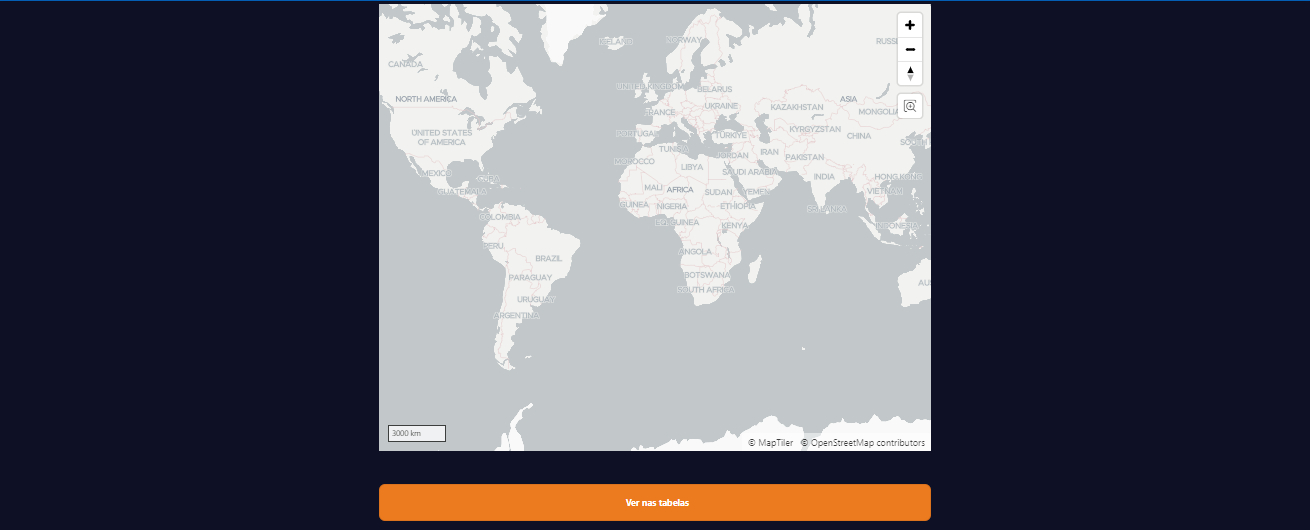
\includegraphics[scale=0.5]{Illustrations/tela3_APEX.png}}
        \usebox0%
        \SourceOrNote{Autoria Própria (2024)}
    \end{figure}

    Ao entrar na tela das Tabelas o usuário pode consultar precisamente a quantidade de plantas infectadas mostradas anteriormente no mapa de calor representado na \Cref{phot:pg-17}.

    \begin{figure}[H]
        \centering
        \SetCaptionWidth{\ifbool{@LayoutA}{0.6}{0.72}\linewidth}
        \caption{Tabelas(APEX)}%
        \label{phot:pg-17}
        \savebox0{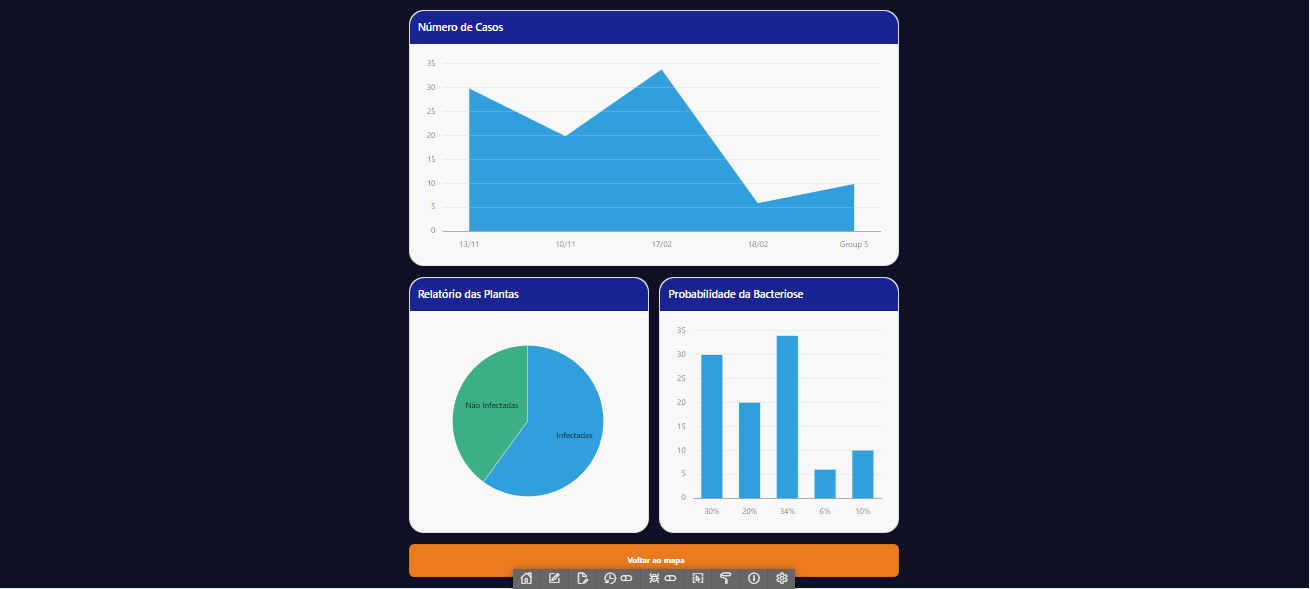
\includegraphics[scale=0.5]{Illustrations/Tela4_APEX.png}}
        \usebox0%
        \SourceOrNote{Autoria Própria (2024)}
    \end{figure}


    \textbf{Diagrama de DCU} 

    Um Diagrama de DCU (ou Diagrama de Casos de Uso) é um tipo de diagrama utilizado na modelagem de sistemas para descrever as interações entre usuários (ou outros sistemas) e o próprio sistema. Seu principal objetivo é demonstrar as diferentes maneiras pelas quais o usuário pode interagir com o sistema, conforme representado na imagem \Cref{phot:pg-12}. Ele faz parte da UML (Unified Modeling Language), uma linguagem de modelagem padrão para representar a estrutura e o comportamento de sistemas de software.

    \begin{figure}[H]
        \centering
        \SetCaptionWidth{\ifbool{@LayoutA}{0.6}{0.72}\linewidth}
        \caption{Diagrama de Caso e Uso (DCU)}%
        \label{phot:pg-12}
        \savebox0{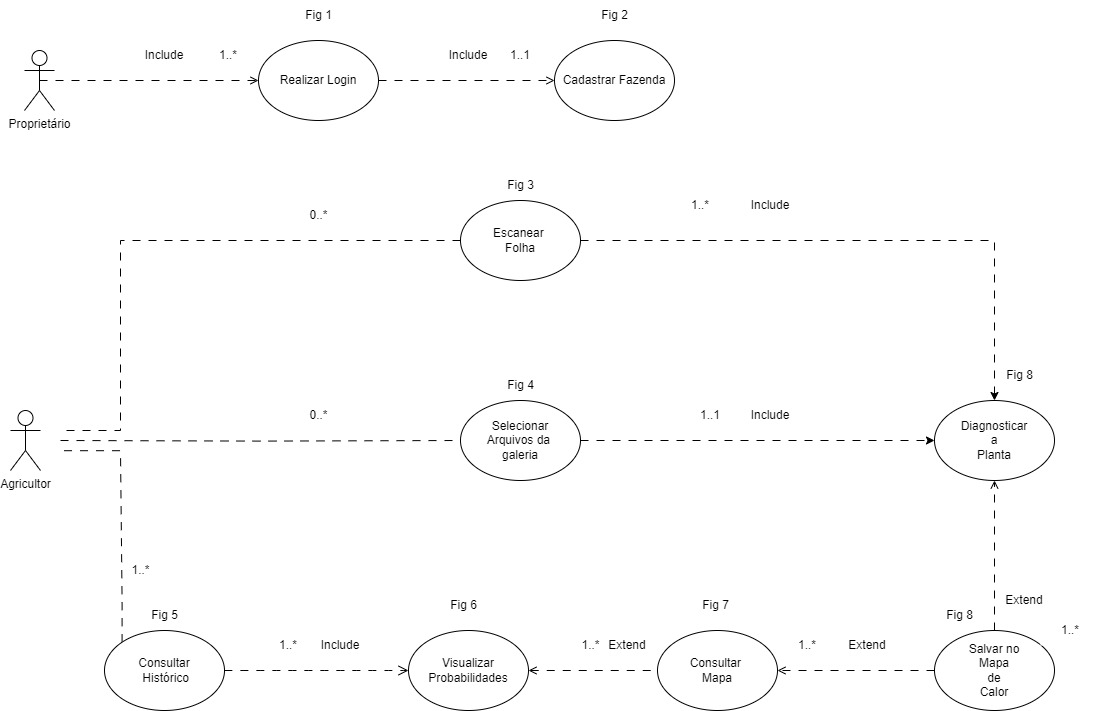
\includegraphics[scale=0.4]{Illustrations/Caso_uso_solo.jpg}}
        \usebox0%
        \SourceOrNote{Autoria Própria (2024)}
    \end{figure}

    \textbf{Modelagem de Banco de Dados (MBD)} \\
    Um modelo relacional é uma abordagem para organizar dados em tabelas, chamadas de relações, onde cada linha representa uma entidade e cada coluna representa um atributo. Ele utiliza chaves primárias para identificar registros de forma única e chaves estrangeiras para estabelecer relações entre as tabelas. Esse modelo é a base dos sistemas de gerenciamento de banco de dados relacionais (SGBD), como mostrado na \Cref{phot:pg-13}. 
    \begin{figure}[H]
        \centering
        \SetCaptionWidth{\ifbool{@LayoutA}{0.6}{0.72}\linewidth}
        \caption{Modelo Conceitual(DCU)}%
        \label{phot:pg-13}
        \savebox0{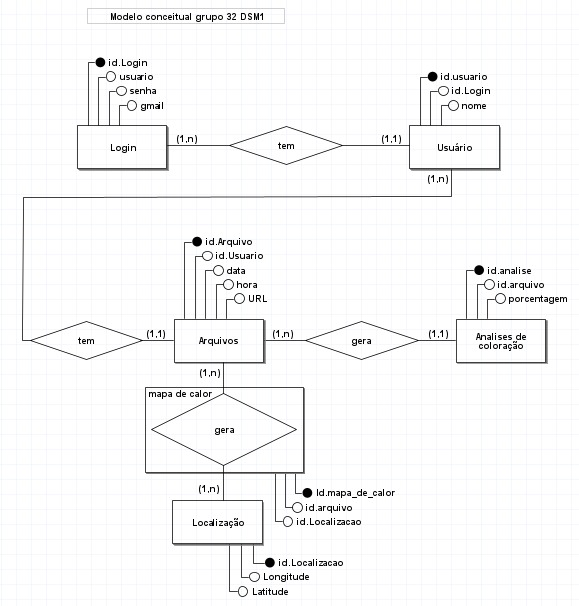
\includegraphics[scale=0.5]{Illustrations/BDC.jpeg}}
        \usebox0%
        \SourceOrNote{Autoria Própria (2024)}
    \end{figure}

    \begin{figure}[H]
        \centering
        \SetCaptionWidth{\ifbool{@LayoutA}{0.6}{0.72}\linewidth}
        \caption{Modelo Lógico(DCU)}%
        \label{phot:pg-14}
        \savebox0{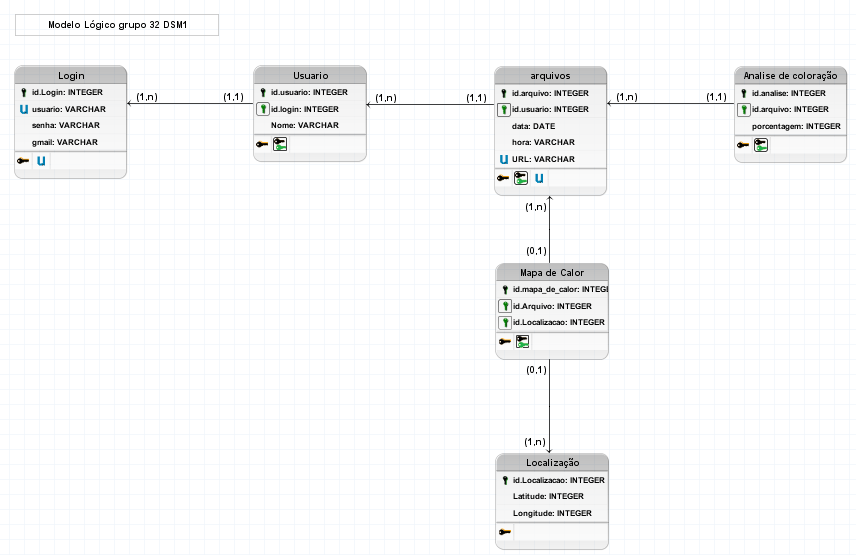
\includegraphics[scale=0.8]{Illustrations/mod_logic1.png}}
        \usebox0%
        \SourceOrNote{Autoria Própria (2024)}
    \end{figure}
    
   Ambos modelos foram criados para mostrar o funcionamento do projeto \textit{Classificação de Bacteriose nas Folhas da Mandioca por Aprendizagem Profunda}, onde o usuário pode tirar fotos, armazená-las e obter uma probabilidade de a planta possuir a bacteriose \textit{Xanthomonas Paesoli}. As entidades \textit{Login} e \textit{Usuário} possibilitam que o usuário entre no sistema. A entidade \textit{Login} possui os seguintes atributos: \textit{id\_login}, como identificador único, \textit{usuario}, como nome do usuário, \textit{senha} e \textit{email}. A entidade \textit{Usuário} possui os atributos: \textit{id\_usuario}, \textit{id\_login} e \textit{nome}. 

    A entidade \textit{Usuário} possui uma relação com a entidade \textit{Arquivos}, que possui os atributos: \textit{id\_arquivo}, para armazenar o ID da foto tirada e sua localização na pasta de arquivos; \textit{id\_usuario}, data, hora e URL, para facilitar a identificação da planta nos registros. 
    
    A entidade \textit{Arquivos} se relaciona com a entidade \textit{Análises de Coloração}, que possui os atributos: \textit{id\_analise}, \textit{id\_arquivo} e \textit{porcentagem}, onde serão armazenadas as informações sobre a porcentagem de bacteriose presente na folha da mandioca. 
    
    A entidade \textit{Arquivos} também se relaciona com a entidade \textit{Localização} essa entidade possui os seguintes atributos: \textit{id\_localização}, \textit{id\_Longitude}, \textit{id\_Latitude}. obs: o relacionamento entre as duas entidades possui cardinalidade n:n ("muitos para muitos"). Para garantir o registro adequado dos dados, utiliza-se uma entidade associativa chamada \textit{Mapa de Calor}, que possui os atributos: \textit{id\_mapa\_de\_calor}, \textit{id\_arquivo} e \textit{id\_localização}. Essa entidade serve para armazenar a localidade do \textit{usuário}.

   
    
    \textbf{Escopo de Redes}
   
    O Escopo de Redes foi montado utilizando uma ferramenta chamada Draw.io, nela foi destacado alguns passos para que o usuário possa utilizar o sistema, mostrando como os dispositivos se comunicam e facilitando o entendimento e a gestão da infraestrutura de rede. \Cref{phot:pg-10}. De inicio cabe ressaltar que o usuário precisa de um celular e acesso a internet para utilizar o nosso serviço, que se localiza na nuvem (optamos por utilizar o serviço AWS). Existem algumas funções fornecidas pelo sistema AWS que  possibilita que o aplicativo funcione. A primeira delas seria o RDS (Relational Database Service) ele funciona como um banco de dados armazenado na nuvem, no qual facilita a configuração, operação e escalabilidade de bancos de dados relacionais. A segunda função seria o RDP  (Remote Desktop Protocol), no qual permite que você acesse um sistema Windows que está hospedado na nuvem de qualquer lugar remotamente; o RDP possui o intuito de treinar a AI (Artificial Intelligence) para que ela gere resultados mais precisos e identifique a bacteriose na folha da mandioca.
    \begin{figure}[H]
        \centering
        \SetCaptionWidth{\ifbool{@LayoutA}{0.6}{0.72}\linewidth}
        \caption{Escopo de Redes}%
        \label{phot:pg-10}
        \savebox0{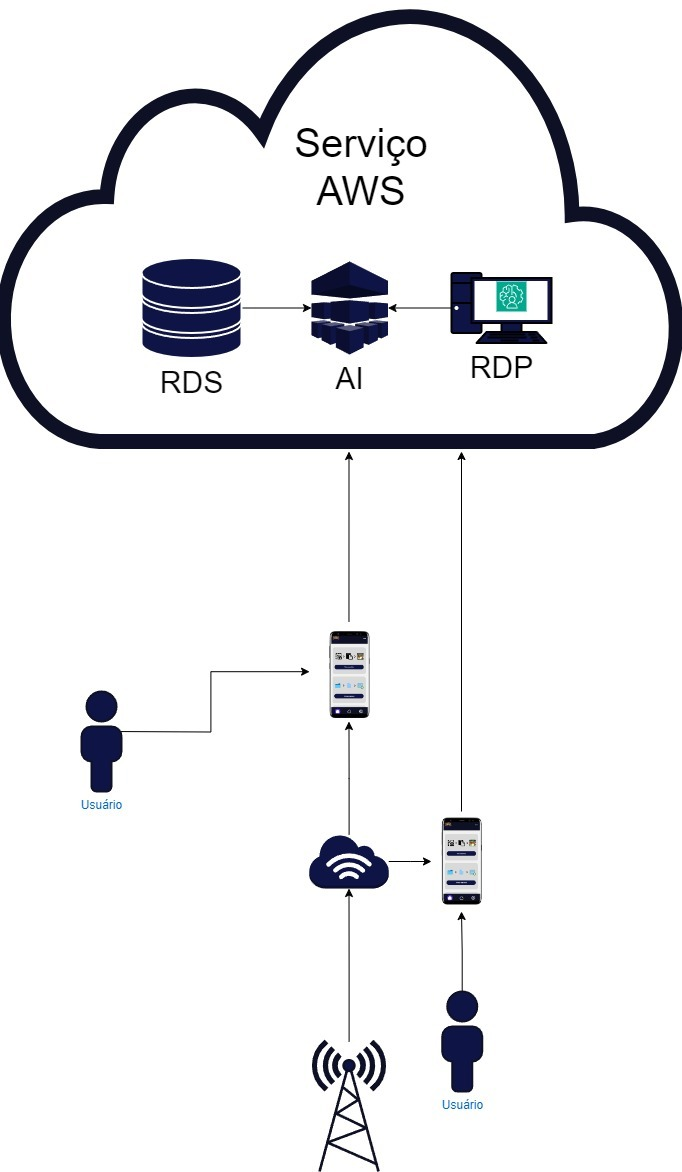
\includegraphics[scale=0.5]{Illustrations/Diagrama_redes.jpg}}
        \usebox0%
        \SourceOrNote{Autoria Própria (2024)}
    \end{figure}

    \textbf{Modelo de Negócios}
    
    Este é um modelo de Business Model Canvas para um aplicativo voltado para a identificação da bacteriose Xanthomonas Phaseoli nas folhas de mandioca, focado principalmente nos agricultores do Vale do Ribeira. 

    Parcerias Chave

    No contexto do projeto, as parcerias chaves incluem pequenmos agricultores locais que visam utilizar da tecnologia para melhorar a qualidade do serviço e também do produto; juntamente da Secretaria de Agricultura dos municípos do Vale do Ribeira. 

    Atividades Chave

    A principal atividade do projeto AVASS é fornecer uma solução automatizada e precisa para identificar a bacteriose nas folhas da mandioca de maneira eficiente e rápida, a fim de minimizar perdas nas colheitas.

    Proposta de Valor

    O aplicativo oferece uma solução para identificar a presença da Xanthomonas Phaseoli nas folhas de mandioca, também possuindo a proposta de preservação da qualidade da mandioca, permitindo que os agricultores façam um monitoramento das áreas mais afetadas com auxilio de um mapa de calor.

    Relacionamento com o Cliente

    O aplicativo oferece suporte direto aos usuários, permitindo que eles descrevam o problema ocorrido e aguardem uma resposta da equipe de suporte; além disso, disponibiliza tutoriais para auxiliar na configuração e uso adequado do sistema, bem como um sistema de feedback onde os usuários podem relatar problemas e sugerir melhorias.

    Segmento de Mercado

    O público-alvo do aplicativo são agricultores de mandioca, especialmente aqueles que cultivam na região do Vale do Ribeira, os quais podem ser diretamente impactados pela bacteriose e, portanto, se beneficiarão do aplicativo para prevenção da bacteriose em suas plantações e suas possíveis perdas.

    Recursos Chave

    O projeto requer programadores para o desenvolvimento e manutenção do aplicativo, funcionários de assistência técnica para auxiliar agricultores e usuários na resolução de problemas técnicos, e uma infraestrutura de hospedagem para armazenamento seguro de dados e realização de análises de forma eficiente (AWS).

    Canais

    Os meios de acesso ao projeto incluem apresentações em feiras e eventos agrícolas, onde ele pode ser demonstrado, além de um site dedicado que atua como canal digital para divulgação e informações sobre o projeto, juntamente com anúncios direcionados ao público que busca soluções para problemas de bacteriose nas plantações de mandioca.

    Estrutura de Custo

    Custo de Manutenção: Inclui despesas gerais como energia e água; Desenvolvimento de Software: Custos relacionados ao desenvolvimento e atualização do aplicativo; Hospedagem: Manutenção de servidores para o site e o aplicativo; Equipamentos: Computadores, monitores, teclados e outros equipamentos necessários para a equipe técnica.

    Fontes de Renda

    O modelo de receita é baseado em assinaturas, onde os usuários pagam uma taxa mensal para acessar o serviço. Isso permite uma receita recorrente e sustentação do projeto. O usuário possuira um teste gratis contendo somente 3 análises, onde respectivamente ele pode tirar somente 3 fotos.

    \begin{figure}[b]
        \centering
        \SetCaptionWidth{\ifbool{@LayoutA}{0.6}{0.72}\linewidth}
        \caption{Modelo de Negócios}%
        \label{phot:pg-11}
        \savebox0{\includegraphics[scale=0.4]{Illustrations/Canva.jpg}}
        \usebox0%
        \SourceOrNote{Autoria Própria (2024)}
    \end{figure}
    


\section*{CONCLUSÃO}\label{sect:conclusao}

Com base nos artigos vistos anteriormente, sabemos que é possível criar um aplicativo que consiga identificar uma bacteriose por meio de uma IA e trazer probabilidades precisas. Quando se trata de analisar imagens e suas complexidades, a Inteligência Artificial se mostra bastante eficaz na geração de informações que podem auxiliar um profissional na avaliação das condições das plantações. Mapas de calor também são possíveis, visto que eles oferecem uma representação visual clara das áreas mais afetadas, facilitando a tomada de decisões estratégicas e otimizando o manejo das culturas. Assim, a integração dessas tecnologias não apenas potencializa a eficiência na identificação de problemas, mas também contribui para a sustentabilidade e produtividade agrícola a longo prazo.


\printbibliography

%% Elementos pós-textuais (opcionais): Apêndice e Anexo
%Caso for utilizar, basta retirar o símbolo de % na frente do comando
%%%%% Elementos pós-textuais
%%
%% Glossário, apêndices, anexos e índice remissivo (opcionais).

%% Apêndices
\begin{Appendix}

\section{Título de Apêndice}%
\label{sect:apx-a1}

Exemplo de apêndice (\Cref{sect:apx-a1}) em uma seção de \nameref{sect:appendix}.

\subsection{Título de Seção Secundária de Apêndice}%
\label{ssect:apx-a2}

Exemplo de seção secundária de apêndice (\Cref{ssect:apx-a2}).

\subsubsection{Título de Seção Terciária de Apêndice}%
\label{sssect:apx-a3}

Exemplo de seção terciária de apêndice (\Cref{sssect:apx-a3}).

\paragraph{Título de seção quaternária de Apêndice}%
\label{prgh:apx-a4}

Exemplo de seção quaternária de apêndice (\Cref{prgh:apx-a4}).

\subparagraph{Título de seção quinária de Apêndice}%
\label{sprgh:apx-a5}

Exemplo de seção quinária de apêndice (\Cref{sprgh:apx-a5}).

\end{Appendix}

%% Anexos
\begin{Annex}

\section{Título de Anexo}%
\label{sect:anx-a1}

Exemplo de anexo (\Cref{sect:anx-a1}) em uma seção de \nameref{sect:annex}.

\subsection{Título de Seção Secundária de Anexo}%
\label{ssect:anx-a2}

Exemplo de seção secundária de anexo (\Cref{ssect:anx-a2}).

\subsubsection{Título de Seção Terciária de Anexo}%
\label{sssect:anx-a3}

Exemplo de seção terciária de anexo (\Cref{sssect:anx-a3}).

\paragraph{Título de seção quaternária de Anexo}%
\label{prgh:anx-a4}

Exemplo de seção quaternária de anexo (\Cref{prgh:anx-a4}).

\subparagraph{Título de seção quinária de Anexo}%
\label{sprgh:anx-a5}

Exemplo de seção quinária de anexo (\Cref{sprgh:anx-a5}).

\end{Annex}

%% Índice remissivo
\printindex%


%% Fim do documento
\end{document}